\documentclass[11pt]{article}

\usepackage{geometry}
\usepackage{natbib}
\usepackage{har2nat}
\usepackage{parskip}
\usepackage{graphicx}
\usepackage{titling}
\usepackage{float}
\usepackage[hidelinks]{hyperref}
\bibliographystyle{abbrv}
\graphicspath{{./images/}}

\renewcommand\maketitlehooka{\null\mbox{}\vfill}
\renewcommand\maketitlehookd{\vfill\null}

\title{Literature Review \\ Active learning of feasible region for porous ceramics}
\date{\today}
\author{Liam LATOUR}

\begin{document}

\begin{titlingpage}
\maketitle
\end{titlingpage}

\tableofcontents
\pagebreak

\section*{Definitions}
\textbf{Porogens}\label{porogen}: Particles, of a specified shape and size, used to make pores in moulded structures used for porous material engineering (they are dissolved away after the structure has set)

\textbf{Aleatoric}\label{aleatoric}: Aleatoric uncertainty refers to the notion of randomness, that is, the variability in the outcome of an experiment which is due to inherently random effects

\textbf{Epistemic}\label{epistemic}: Epistemic uncertainty refers to uncertainty caused by a lack of knowledge, i.e., the lack of data points in the model.

\section{Introduction}
% Provide an overview of the topic, significance, purpose, and objectives of the review.
Ceramic resin composites are composite materials that merge the robustness of ceramics with the flexibility of resins, offering enhanced strength, durability, and versatility. The process involves infusing porous ceramic structures with resin, achieving a remarkable balance of properties crucial for demanding environments. Fabricated through techniques such as sintering\cite{leriche_sintering_2017} or additive manufacturing, these composites undergo processes such as vacuum impregnation or resin transfer molding, ensuring homogeneity and reinforcing the structure with added toughness and ductility. Widely applicable across industries including aerospace, automotive and medical, ceramic resin composites revolutionize engineering by enabling the development of lightweight yet high-performance components.

To create the porous ceramic through sintering\cite{ha_effect_2013}, porogens (often in the form of plastic beads) are added to the ceramic powder before applying pressure. The porogens are then removed by heating, which leaves a hopefully porous, yet cohesive, ceramic matrix behind. This ceramic matrix is then sintered to solidify it before infusion.

Porogen size distribution and total volume plays a huge role in the porosity of the final material and thus the resin to ceramic ratio. Furthermore, adding too much porogens can break the material before sintering, rendering it useless. This is why knowing which porogen mix will not break (the feasible region) beforehand is crucial to efficient manufacturing.

Discovering the feasible region is done through testing samples of various porogen distributions, unfortunately each test is quite costly in time so exploring blindly is not very effective. This is where active learning comes in. Active learning is a subfield of machine learning which goal it is to optimise which candidate sample has to be tested to improve the more the model.

This review will focus on the literature surrounding active learning and the various modeling methods it can rely on, applied to our specific problem.

\section{Active learning framework}
In the realm of machine learning, the active learning framework presents a strategic paradigm where the algorithm autonomously selects the most informative instances from an unlabeled dataset for annotation by an oracle, typically a human expert, in our case testing the actual porogen mix\cite{settles_active_2009}. This iterative process aims to optimize model 
performance with minimal labeled data, effectively reducing annotation costs and number of required data points. Through sequential queries, the algorithm strategically selects instances that are most uncertain or likely to improve the model's performance, thus actively guiding the learning process. Active learning finds applications across various domains, including text classification, image recognition, and medical diagnostics, where labeled data is scarce or expensive to obtain. Its ability to prioritize data selection based on information gain has rendered it instrumental in improving the efficiency and efficacy of machine learning models, particularly in scenarios where labeled data is limited or costly.

\begin{figure}[H]
  \centering
  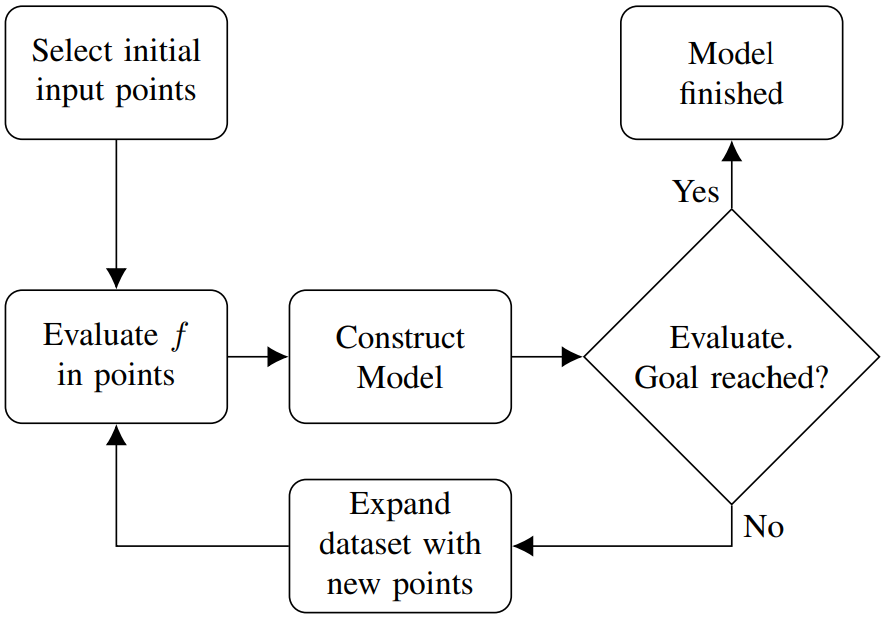
\includegraphics[width=0.7\textwidth]{ActiveLearning.png}
  \caption{Active learning flow chart}\label{fig:active}
\end{figure}

Active learning is always added on top of a modeling method that it improves through the iterative process. Usually it also uses outputs from the underlying method to make its decision on the next data point to test. This decision is based on information theory and the goal is to reduce the uncertainty of the model. To be more precise we want to reduce the epistemic uncertainty and ideally ignore aleatoric variance which is only the non deterministic aspect of the process. The underlying model used by active learning has to, not only, output a predicted value for a given data point but also an estimation of the uncertainty attributed to this prediction. The goal of active learning
is to find the test point that maximises model uncertainty thus maximizing the estimated learning gained from knowing it.

\section{Methods for choosing the best candidate point}
% Estimated Error, Model change, entropy, ...
Uncertainty of a given prediction can be computed in various ways and this impacts the selection of the interest point. Usual methods are: uncertainty sampling, estimated error, expected model change.%, variance reduction.

\subsection{Uncertainty sampling}
Uncertainty sampling is a query framework commonly used in active learning, where the learner selects instances for labeling based on the uncertainty of their predicted labels. The simplest form, queries instances where the model is least certain about the label, typically calculated using probabilities from the model\cite{lewis_sequential_1994}.
For binary classification, this means querying instances with a posterior probability as close to 0.5 as possible. For problems with multiple classes, variants like least confident, margin, and entropy sampling are used. Least confident queries the instance with the lowest probability for the predicted label, margin considers the difference between the top two probable labels, and entropy measures uncertainty using information entropy.

Empirical studies comparing these methods have shown mixed results, suggesting that the best strategy depends on the application\cite{hutchison_multi-class_2006}\cite{schein_active_2004}. However, entropy sampling is suitable for minimizing log-loss, while least confident and margin sampling are better for reducing classification error.

Uncertainty sampling is not limited to probabilistic classifiers; it can be applied to non-probabilistic classifiers like decision trees and support vector machines. It's also applicable to regression problems, where the learner selects instances based on the model's highest output variance prediction.

Overall, uncertainty sampling is a versatile approach in active learning, offering various strategies to select informative instances for labeling across different types of learning tasks.

\subsection{Estimated error}
Expected Error Reduction (EER) is a decision-theoretic approach in active learning that focuses on reducing the model's generalization error. Instead of considering how much the model's predictions might change, EER estimates the expected future error of a model trained on the current labeled data and queries the instance that is expected to minimize this future error the most.

One way to implement EER is by minimizing the expected 0/1-loss, which involves estimating the total number of incorrect predictions expected when the model is trained with the queried instance. Another approach is to minimize the expected log-loss, which is equivalent to reducing the expected entropy over the unlabeled instances. This strategy aims to maximize the expected information gain from querying a specific instance\cite{zhao_efficient_2021}.

EER was first proposed for text classification tasks using naïve Bayes models, and it has been combined with semi-supervised learning approaches to achieve significant improvements over random or uncertainty sampling. Variants of EER exist, such as an ``optimistic'' variant that biases expectations toward the most likely label for computational convenience, while still resorting to uncertainty sampling when necessary.

EER can be applied across various model classes, including naïve Bayes, Gaussian random fields, logistic regression, and support vector machines. However, it is computationally expensive because it requires estimating future errors for each query and retraining the model incrementally for each possible labeling of the queried instance. This computational complexity limits its practicality, especially for models with large parameter spaces or complex structures.

Efforts to address the computational burden of EER include Monte Carlo sampling from the pool of unlabeled instances and the use of approximate training techniques to reduce the number of gradient computations. Despite these challenges, EER remains a powerful approach, particularly for simple binary classification tasks where the computational overhead is more manageable.

\subsection{Model change}
Expected Model Change (EMC) is an active learning framework that employs a decision-theoretic strategy to select instances that would cause the most significant change to the current model if their labels were known. One approach within this framework is the ``expected gradient length'' (EGL) strategy, particularly applicable to discriminative probabilistic models trained using gradient-based optimization\cite{settles_multiple-instance_2007}.

The EGL strategy focuses on measuring the change induced in the model parameters by considering the length of the training gradient, which represents the vector used to update parameter values during training. The instance chosen for labeling is the one expected to yield the largest magnitude change in the gradient if its label were known and it were added to the labeled set\cite{cai_active_2014}.

To calculate the expected gradient length, the algorithm estimates the gradient length as an expectation over all possible labelings, considering the likelihood of each label given the instance. This approach aims to select instances that are likely to have the most influence on the model's parameters, irrespective of the specific label assigned.

While the EGL strategy has shown effectiveness in empirical studies, it can be computationally intensive, especially for large feature spaces and label sets. Additionally, improperly scaled features may lead to misleadingly high gradient magnitudes, potentially affecting the informativeness of selected instances. However, techniques like parameter regularization can mitigate this issue to some extent.

Overall, EMC, particularly through the EGL approach, provides a principled method for selecting informative instances that can significantly impact the model's parameters, contributing to improved model performance in active learning scenarios.

\section{Different modeling methods}
The active learning framework relies on an underlying model which heavily impacts the implementation and results. Therefore it is crucial to understand the differences between the most used models in the literature.

\subsection{Gaussian Process}
Gaussian process is the most explored model in literature, and a very versatile framework\cite{rasmussen_gaussian_2005}. It can either be used for regression or classification. The major interest of Gaussian Processes is that they output uncertainty without needing any extra step. The classification version is often derived from a regression passed through a sigmoid function to bound output between 0--1, unfortunately the variance can not be extracted from this version\cite{jensen_bounded_2013}\cite{nickisch_approximations_2008}\cite{snelson_warped_2003}.

\begin{figure}[H]
  \centering
  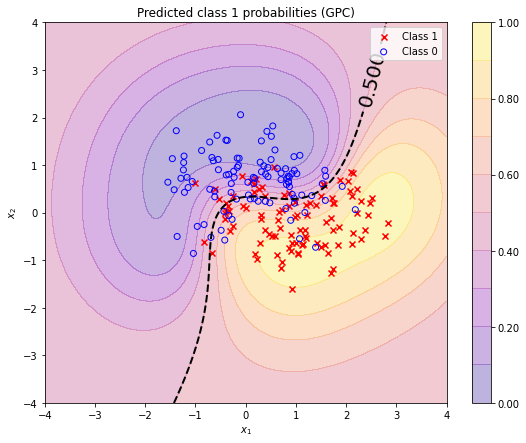
\includegraphics[width=0.7\textwidth]{GPC.png}
  \caption{2D GP for a classification task}\label{fig:gpc}

  Color is predicted class (below 0.5 is 0 with uncertainty equal to the predicted value, and vice versa for above 0.5)

  The dotted line represents the boundary between classes
\end{figure}

Gaussian Processes (GPs) are well-known for their effectiveness in regression and uncertainty estimation tasks. They provide a structured way to understand complex connections between different factors and to determine how confident we are in future predictions. This is especially useful in situations where making informed decisions relies on accurate uncertainty estimation. By using the probabilities provided by GPs, practitioners can decide which samples to label first. Samples that GPs are less certain about are given priority for labeling, which helps improve predictive models and decision-making. Additionally, GPs are versatile and can handle various types of data and problems. They are also computationally efficient, especially with smaller datasets, making them suitable for scalable active learning approaches\cite{kapoor_active_2007}. Integrating Gaussian Processes into active learning methods improves model performance by selecting the most informative examples for labeling, highlighting their importance in advancing machine learning research and practical applications.

\subsection{Support Vector Margins}
In the realm of active learning methodologies, Support Vector Machine (SVM) modeling stands out as a powerful technique known for its efficacy in classification tasks. SVMs excel in finding decision boundaries in high-dimensional feature spaces by maximizing the margin between classes, thereby enhancing generalization performance. When integrated into active learning frameworks, SVMs offer a robust approach to selecting informative instances for labeling\cite{kremer_active_2014}. Additionally, SVMs can heavily benefit from the ``kernel trick'' which transforms the n-dimensional problem into a higher dimensionality thus removing the inherent linearity of SVMs.
\begin{figure}[H]
  \centering
  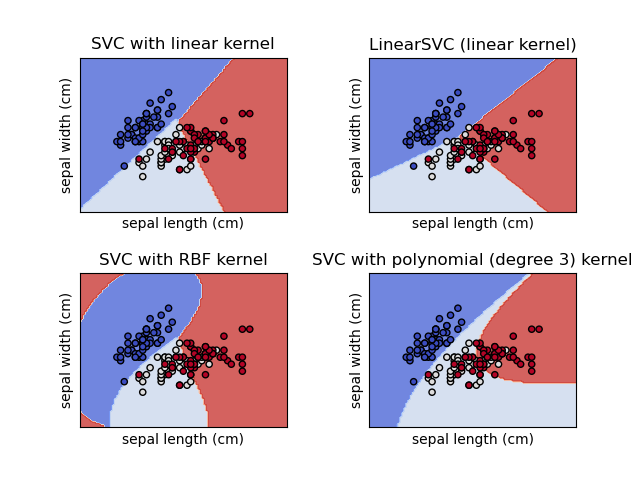
\includegraphics[width=0.7\textwidth]{SVM.png}
  \caption{SVM with different kernels, using the ``kernel trick''}\label{fig:svm}
\end{figure}
By leveraging their inherent capacity to identify support vectors—instances crucial for defining the decision boundary—SVMs can effectively assess the uncertainty associated with predictions. This uncertainty estimation serves as a pivotal criterion for prioritizing instances for labeling in active learning scenarios. Instances with heightened uncertainty are deemed more informative and are thus given precedence for annotation, enabling the model to refine its decision boundary with optimal efficiency. Furthermore, SVMs boast computational efficiency, particularly in scenarios involving sparse data or high-dimensional feature spaces, rendering them amenable to scalable active learning implementations. Consequently, the amalgamation of SVM modeling with active learning strategies represents a pragmatic approach to expedite model convergence and enhance predictive accuracy through judicious instance selection for labeling.

\subsection{Random Forest}
Random Forest stands as a prominent ensemble learning method renowned for its robustness and versatility. By aggregating predictions from numerous decision trees, each trained on bootstrapped subsets of the training data and utilizing random subsets of features, Random Forest offers a reliable framework for predictive modeling.
\begin{figure}[H]
  \centering
  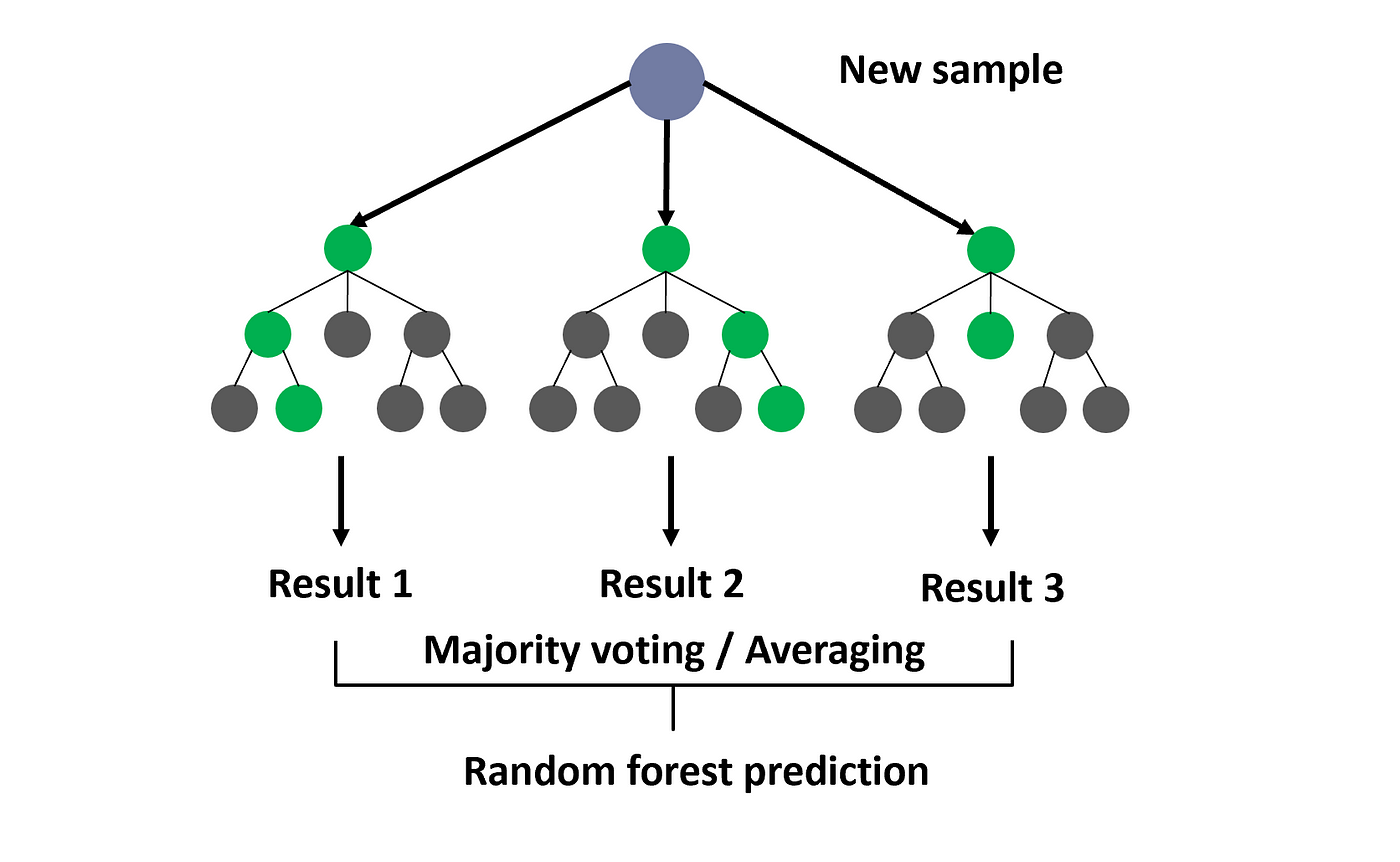
\includegraphics[width=0.7\textwidth]{RF.png}
  \caption{Random forest principle}\label{fig:rf}
\end{figure}
In active learning contexts, its ensemble nature enables effective estimation of prediction uncertainty. Through the synthesis of predictions from diverse trees, Random Forest can accurately gauge the variability in predicted labels for individual instances, facilitating informed decision-making regarding instance selection for labeling\cite{gu_active_2015}. This capability is particularly valuable in active learning scenarios, where the strategic allocation of labeling resources is essential. By prioritizing instances with elevated uncertainty, active learning algorithms optimize the information gained from each labeled sample. Furthermore, Random Forest's computational efficiency ensures its practical applicability in scalable active learning implementations, even with large datasets. Consequently, the integration of Random Forest into active learning methodologies offers a pragmatic approach to enhancing model convergence and predictive performance.


\section{Specificities of our problem}
% information density, can explore the full space, active learning is more suited for AI purposes
Usually the active learning framework is used to train AIs to optimize the labellisation of more usefull samples. This implies that the candidate points are predetermined which is not the same in our case as we can choose to test any point in the feature space. Furthermore, in the context of training AIs we usually prefer to label data close to the most probable sample, in our case we want to do the opposite, we want to learn the whole boundary of feasible space, which implies choosing points far from the previous ones. This is known as a feasible region discovery as in~\cite[Knudde (2019)]{knudde_active_2019}.

\subsection{Continuous space sampling}
% explore the fact that we can choose anything
In the realm of Active Learning, sampling instances for labeling becomes particularly challenging when dealing with continuous feature spaces. Unlike discrete feature spaces where instances are finite and enumerable, continuous spaces pose a unique set of obstacles due to their infinite nature. Sampling in continuous spaces requires careful consideration to ensure representative coverage and effective exploration. Traditional random sampling methods may not suffice in continuous spaces as they can overlook regions of high uncertainty or importance. Therefore, specialized sampling strategies tailored to continuous spaces are essential to maximize the informativeness of labeled instances. Techniques such as uncertainty-based sampling, density estimation, and gradient-based methods offer avenues for intelligently selecting instances for labeling in continuous spaces. However, the computational complexity and scalability of these methods remain significant challenges, especially in high-dimensional spaces. Addressing the problem of continuous space sampling in Active Learning is crucial for enhancing the efficiency and effectiveness of the labeling process, ultimately leading to improved model performance and decision-making.

\subsection{Density aware sampling}
% density shit
Usually, data density is used to focus the candidate selection on high density data\cite{settles_analysis_2008}.
In our case, density-aware sampling involves selecting instances for labeling based on the density of the data distribution. Unlike random sampling, which treats all instances equally, density-aware sampling prioritizes regions of the feature space where the data density is low. This approach aims to explore and exploit regions of uncertainty or sparsity, which are often indicative of areas where the model could benefit the most from additional labeled data. Density-aware methods, such as cluster-based sampling or kernel density estimation, enable the identification of regions where the model's uncertainty is high or where the data distribution is underrepresented. By focusing labeling efforts on these informative regions, density-aware sampling strategies can lead to more efficient model improvement compared to random sampling. However, challenges remain in efficiently estimating data density in high-dimensional spaces and adapting density-aware methods to different problem domains. Nonetheless, density-aware sampling represents a promising avenue for enhancing the effectiveness of Active Learning by intelligently selecting instances for labeling based on the underlying data distribution.

\subsection{Single or batch point sampling}
% talk about the dilemma of single or multi point
In the domain of Active Learning, the strategy of single or multi-point sampling pertains to the selection of individual instances or batches of instances for labeling, respectively. Single-point sampling involves choosing one instance at a time for labeling, typically based on certain criteria such as uncertainty estimation, diversity, or representativeness. This approach allows for fine-grained control over the labeling process, enabling the model to focus on specific areas of uncertainty or interest. On the other hand, multi-point sampling involves selecting multiple instances simultaneously for labeling, often in batches. This approach leverages the efficiency gained from labeling multiple instances at once\cite{brinker_incorporating_2003}\cite{xu_incorporating_2007}, allowing for faster model improvement and better exploration of the feature space. Both single and multi-point sampling strategies have their advantages and trade-offs. Single-point sampling offers flexibility and adaptability, making it suitable for scenarios where instances are selected based on dynamic criteria or where labeling resources are limited. Conversely, multi-point sampling enhances efficiency by leveraging batch processing capabilities, particularly in large-scale or resource-intensive applications. Choosing between single or multi-point sampling depends on factors such as the specific task requirements, computational resources, and the desired balance between exploration and exploitation in the Active Learning process.

\section{Conclusion}
% Summarize main findings, highlight significance, suggest future research directions, and conclude with a closing statement.
In conclusion, Active Learning encompasses a diverse array of strategies and methodologies aimed at optimizing the process of labeling instances to improve machine learning models. From uncertainty sampling to density-aware sampling, and from single-point to multi-point sampling, the field offers a rich tapestry of techniques designed to tackle various challenges encountered in different learning scenarios. These approaches, whether based on probabilistic models like Gaussian Processes or discriminative models like Support Vector Machines, are united by their common goal of maximizing the informativeness of labeled data to enhance model performance and efficiency. While each method has its strengths and limitations, the overarching aim remains consistent: to iteratively refine models through strategic selection of instances for labeling, thereby reducing annotation costs, accelerating model convergence, and ultimately advancing the state-of-the-art in machine learning.

In the case of my problem, I will begin by focusing on Gaussian Process with model change and density aware methods, as this seems to be the closest to what is needed. In a second time I will focus on comparing the original results with a SVM and random forest approach. Finally, I will try adding a batch sampling method to improve overall efficacy.

%\nocite{*}
\bibliography{references} % Include your bibliography file

\end{document}
